%%%%%%%%%%%%%%%%%%%%%%%%%%%%%%%%%%%%%%%%%
% Programming/Coding Assignment
% LaTeX Template
%
% This template has been downloaded from:
% http://www.latextemplates.com
%
% Original author:
% Ted Pavlic (http://www.tedpavlic.com)
%
% Note:
% The \lipsum[#] commands throughout this template generate dummy text
% to fill the template out. These commands should all be removed when 
% writing assignment content.
%
% This template uses a Perl script as an example snippet of code, most other
% languages are also usable. Configure them in the "CODE INCLUSION 
% CONFIGURATION" section.
%
%%%%%%%%%%%%%%%%%%%%%%%%%%%%%%%%%%%%%%%%%

%----------------------------------------------------------------------------------------
%	PACKAGES AND OTHER DOCUMENT CONFIGURATIONS
%----------------------------------------------------------------------------------------

\documentclass{article}

\usepackage[utf8]{inputenc}
\usepackage{fancyhdr} % Required for custom headers
\usepackage{lastpage} % Required to determine the last page for the footer
\usepackage{extramarks} % Required for headers and footers
\usepackage[usenames,dvipsnames]{color} % Required for custom colors
\usepackage{graphicx} % Required to insert images
\usepackage{listings} % Required for insertion of code
\usepackage{courier} % Required for the courier font
\usepackage{lipsum} % Used for inserting dummy 'Lorem ipsum' text into the template

% Margins
\topmargin=-0.45in
\evensidemargin=0in
\oddsidemargin=0in
\textwidth=6.5in
\textheight=9.0in
\headsep=0.25in

\linespread{1.1} % Line spacing

% Set up the header and footer
\pagestyle{fancy}
\lhead{\hmwkAuthorName} % Top left header
\chead{\hmwkClass\ (\hmwkClassInstructor\ \hmwkClassTime): \hmwkTitle} % Top center head
\rhead{\firstxmark} % Top right header
\lfoot{\lastxmark} % Bottom left footer
\cfoot{} % Bottom center footer
\rfoot{Page\ \thepage\ of\ \protect\pageref{LastPage}} % Bottom right footer
\renewcommand\headrulewidth{0.4pt} % Size of the header rule
\renewcommand\footrulewidth{0.4pt} % Size of the footer rule

\setlength\parindent{0pt} % Removes all indentation from paragraphs

%----------------------------------------------------------------------------------------
%	CODE INCLUSION CONFIGURATION
%----------------------------------------------------------------------------------------

\definecolor{MyDarkGreen}{rgb}{0.0,0.4,0.0} % This is the color used for comments
\lstloadlanguages{Perl} % Load Perl syntax for listings, for a list of other languages supported see: ftp://ftp.tex.ac.uk/tex-archive/macros/latex/contrib/listings/listings.pdf
\lstset{language=Perl, % Use Perl in this example
        frame=single, % Single frame around code
        basicstyle=\small\ttfamily, % Use small true type font
        keywordstyle=[1]\color{Blue}\bf, % Perl functions bold and blue
        keywordstyle=[2]\color{Purple}, % Perl function arguments purple
        keywordstyle=[3]\color{Blue}\underbar, % Custom functions underlined and blue
        identifierstyle=, % Nothing special about identifiers                                         
        commentstyle=\usefont{T1}{pcr}{m}{sl}\color{MyDarkGreen}\small, % Comments small dark green courier font
        stringstyle=\color{Purple}, % Strings are purple
        showstringspaces=false, % Don't put marks in string spaces
        tabsize=5, % 5 spaces per tab
        %
        % Put standard Perl functions not included in the default language here
        morekeywords={rand},
        %
        % Put Perl function parameters here
        morekeywords=[2]{on, off, interp},
        %
        % Put user defined functions here
        morekeywords=[3]{test},
       	%
        morecomment=[l][\color{Blue}]{...}, % Line continuation (...) like blue comment
        numbers=left, % Line numbers on left
        firstnumber=1, % Line numbers start with line 1
        numberstyle=\tiny\color{Blue}, % Line numbers are blue and small
        stepnumber=5 % Line numbers go in steps of 5
}

% Creates a new command to include a perl script, the first parameter is the filename of the script (without .pl), the second parameter is the caption
\newcommand{\perlscript}[2]{
\begin{itemize}
\item[]\lstinputlisting[caption=#2,label=#1]{#1.pl}
\end{itemize}
}

%----------------------------------------------------------------------------------------
%	DOCUMENT STRUCTURE COMMANDS
%	Skip this unless you know what you're doing
%----------------------------------------------------------------------------------------

% Header and footer for when a page split occurs within a problem environment
\newcommand{\enterProblemHeader}[1]{
\nobreak\extramarks{#1}{#1 continued on next page\ldots}\nobreak
\nobreak\extramarks{#1 (continued)}{#1 continued on next page\ldots}\nobreak
}

% Header and footer for when a page split occurs between problem environments
\newcommand{\exitProblemHeader}[1]{
\nobreak\extramarks{#1 (continued)}{#1 continued on next page\ldots}\nobreak
\nobreak\extramarks{#1}{}\nobreak
}

\setcounter{secnumdepth}{0} % Removes default section numbers
\newcounter{homeworkProblemCounter} % Creates a counter to keep track of the number of problems

\newcommand{\homeworkProblemName}{}
\newenvironment{homeworkProblem}[1][Task \arabic{homeworkProblemCounter}]{ % Makes a new environment called homeworkProblem which takes 1 argument (custom name) but the default is "Problem #"
\stepcounter{homeworkProblemCounter} % Increase counter for number of problems
\renewcommand{\homeworkProblemName}{#1} % Assign \homeworkProblemName the name of the problem
\section{\homeworkProblemName} % Make a section in the document with the custom problem count
\enterProblemHeader{\homeworkProblemName} % Header and footer within the environment
}{
\exitProblemHeader{\homeworkProblemName} % Header and footer after the environment
}

\newcommand{\problemAnswer}[1]{ % Defines the problem answer command with the content as the only argument
\noindent\framebox[\columnwidth][c]{\begin{minipage}{0.98\columnwidth}#1\end{minipage}} % Makes the box around the problem answer and puts the content inside
}

\newcommand{\homeworkSectionName}{}
\newenvironment{homeworkSection}[1]{ % New environment for sections within homework problems, takes 1 argument - the name of the section
\renewcommand{\homeworkSectionName}{#1} % Assign \homeworkSectionName to the name of the section from the environment argument
\subsection{\homeworkSectionName} % Make a subsection with the custom name of the subsection
\enterProblemHeader{\homeworkProblemName\ [\homeworkSectionName]} % Header and footer within the environment
}{
\enterProblemHeader{\homeworkProblemName} % Header and footer after the environment
}

%----------------------------------------------------------------------------------------
%	NAME AND CLASS SECTION
%----------------------------------------------------------------------------------------

\newcommand{\hmwkTitle}{Report\ \#2} % Assignment title
\newcommand{\hmwkDueDate}{Monday,\ June\ 2,\ 2014} % Due date
\newcommand{\hmwkClass}{INEA00104L} % Course/class
\newcommand{\hmwkClassTime}{} % Class/lecture time
\newcommand{\hmwkClassInstructor}{Mgr inż. Andrzej Wytyczak-Partyka} % Teacher/lecturer
\newcommand{\hmwkAuthorName}{inż. Piotr Giedziun} % Your name

%----------------------------------------------------------------------------------------
%	TITLE PAGE
%----------------------------------------------------------------------------------------

\title{
\vspace{2in}
\textmd{\textbf{\hmwkClass:\ \hmwkTitle}}\\
\normalsize\vspace{0.1in}\small{Due\ on\ \hmwkDueDate}\\
\vspace{0.1in}\large{\textit{\hmwkClassInstructor\ \hmwkClassTime}}
\vspace{3in}
}

\author{\textbf{\hmwkAuthorName}}
\date{} % Insert date here if you want it to appear below your name

%----------------------------------------------------------------------------------------

\begin{document}

\maketitle

%----------------------------------------------------------------------------------------
%	TABLE OF CONTENTS
%----------------------------------------------------------------------------------------

%\setcounter{tocdepth}{1} % Uncomment this line if you don't want subsections listed in the ToC

\newpage

\section{Introduction}
This report was made to present results of work done during last class.
Main goal of this paper it to document different aspects of indexing performance.

%----------------------------------------------------------------------------------------
%	TASK 1
%----------------------------------------------------------------------------------------

\begin{homeworkProblem}
Why is MySQL choosing a full table scan instead of using index on price column when doing a SELECT * FROM tickets ORDER BY price?
\newline\newline
Quick reminder of `ticket` table structure.
\begin{lstlisting}[language=SQL] 
mysql> SHOW COLUMNS FROM sakila.ticket;
+----------------------+----------------------+------+-----+---------+----------------+
| Field                | Type                 | Null | Key | Default | Extra          |
+----------------------+----------------------+------+-----+---------+----------------+
| ticket_id            | int(11)              | NO   | PRI | NULL    | auto_increment |
| price                | float                | NO   | MUL | NULL    |                |
| seat_seat_id         | int(11)              | NO   | MUL | NULL    |                |
| show_show_id         | int(11)              | NO   | MUL | NULL    |                |
| cinema_cinema_id     | int(11)              | NO   | MUL | NULL    |                |
| customer_customer_id | smallint(5) unsigned | YES  | MUL | NULL    |                |
| theater_id           | int(11)              | NO   | MUL | NULL    |                |
+----------------------+----------------------+------+-----+---------+----------------+
7 rows in set (0.00 sec)
\end{lstlisting}


We were ask to add index on price column. 
\begin{lstlisting}[language=SQL] 
mysql> ALTER TABLE sakila.ticket ADD INDEX price_idx (price);
\end{lstlisting}

Following query should take advantage of price\_idx index, with should result in full index scan.

\begin{lstlisting}[language=SQL] 
mysql> EXPLAIN SELECT SQL_NO_CACHE * FROM sakila.ticket ORDER BY price;
\end{lstlisting}

\begin{figure}[ht!]
\centering
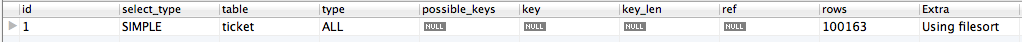
\includegraphics[width=1.0\columnwidth]{query_1} 
\end{figure}

This result looks surprising, MySQL optimizer decided to do a full table scan (Using filesort, key=NULL).
Let's try do another one, this time I will force optimizer to use index.

\begin{lstlisting}[language=SQL] 
mysql> EXPLAIN SELECT SQL_NO_CACHE * FROM sakila.ticket FORCE INDEX(price_idx)
	ORDER BY price;
\end{lstlisting}

\begin{figure}[ht!]
\centering
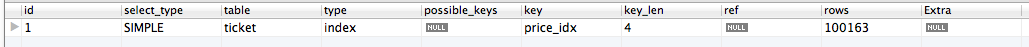
\includegraphics[width=1.0\columnwidth]{query_2} 
\end{figure}

This time around we are doing full index scan (key=price\_idx). Number of rows is exactly the same as previous. Both cases are performing full scan.
\newline\newline
In order to understand the difference we have to understand, how MySQL is storing data. 
When we are doing full table scan, MySQL is performing sequential reads of stored data. However, when we are doing full index scan, MySQL have to perform a lot of random reads (reading data pointed by index). 

In this case full table scan is just faster than full index scan. I did few tests on my local machine in order to confirm it.
Unlucky, I have SSD drive, so random read is not a problem for this hardware architecture.
MySQL optimizer decided to use full table scan by default because this method should be faster (generaly speaking).

It also explain why MySQL optimizer used full index scan for following query.

\begin{lstlisting}[language=SQL] 
mysql> EXPLAIN SELECT price FROM sakila.ticket ORDER BY price;
\end{lstlisting}

\begin{figure}[ht!]
\centering
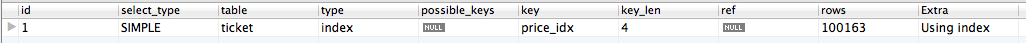
\includegraphics[width=1.0\columnwidth]{query_3} 
\end{figure}

This time around there is no need for random data access. All data we asked is stored in indexing structure. We don't have to use indexing pointer anymore.
\end{homeworkProblem}

%----------------------------------------------------------------------------------------
%	PROBLEM 2
%----------------------------------------------------------------------------------------

\begin{homeworkProblem}
Performance issues involved with using indexes on VARCHAR fields.
How does prefixing them influence index size and QPS
\newline\newline
This issue was explained in my previous report.
\end{homeworkProblem}

%----------------------------------------------------------------------------------------
%	PROBLEM 3
%----------------------------------------------------------------------------------------

\begin{homeworkProblem}
Explain why EXPLAIN SELECT SQL\_NO\_CACHE * FROM sakila.ticket ORDER BY theater\_id DESC is not using theater\_id\_price\_idx
\newline\newline
This issue was explained in Task 1 section.
\newline\newline
TL;DR: MySQL optimizer decided to use full table scan, because it's faster than full index scan. Sequential reads are performed faster than random reads (on default HD drive).

\end{homeworkProblem}

\begin{homeworkProblem}
Explain why EXPLAIN SELECT ticket.price FROM ticket LEFT JOIN theater on theater.theater\_id = ticket.theater\_id ORDER BY ticket.price DESC is not using price\_idx INDEX.
\newline\newline
This query is also related with Task 1. I was looking for an answer on MySQL doc, but I didn't found one.
What I'm about to say is pure guess. I will try to support it with evidence.
\newline\newline
First, let's execute following query.
\begin{lstlisting}[language=SQL] 
mysql> EXPLAIN SELECT ticket.price FROM ticket LEFT JOIN theater
	on theater.theater_id = ticket.theater_id ORDER BY ticket.price;
\end{lstlisting}

\begin{figure}[ht!]
\centering
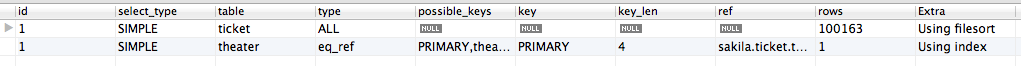
\includegraphics[width=1.0\columnwidth]{query_4} 
\end{figure}

My first guess was, that this query will use price\_idx index.
Query looks similar to SELECT price FROM sakila.ticket ORDER BY price (explained in Task 1 section).
MySQL decided to use full file sort, because it's faster that full index sort (also explained in Task 1 section).
The question is: Why it differs from SELECT price FROM sakila.ticket ORDER BY price, while using JOIN?

\begin{lstlisting}[language=SQL] 
mysql> SELECT price FROM sakila.ticket ORDER BY price;
\end{lstlisting}
\begin{figure}[ht!]
\centering
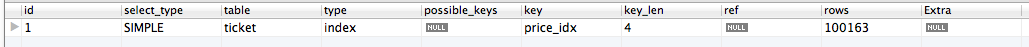
\includegraphics[width=1.0\columnwidth]{query_2} 
\end{figure}
This query will return all prices values. This data is stored in index structure. MySQL will use full index scan, because it does not requires additional random reads (all data is already provided).
However, if we will return additional field, who's not a part of index, MySQL will perform full table scan.

\begin{lstlisting}[language=SQL] 
mysql> SELECT theater_id, price FROM sakila.ticket ORDER BY price;
\end{lstlisting}
\begin{figure}[ht!]
\centering
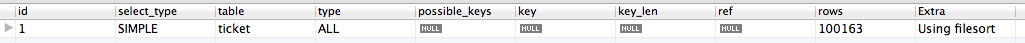
\includegraphics[width=1.0\columnwidth]{query_5} 
\end{figure}

\begin{lstlisting}[language=SQL] 
mysql> EXPLAIN SELECT ticket.price FROM ticket LEFT JOIN theater
	on theater.theater_id = ticket.theater_id ORDER BY ticket.price;
\end{lstlisting}

Using LEFT JOIN forced MySQL to look for ticket.theater\_id. Instead of "SELECT ticket.price" it's "SELECT ticket.theater\_id, ticket.price".
\newline\newline
In order to make it more reliable, I decided to crate new index, containing both fields (price and theater\_id).

\begin{lstlisting}[language=SQL] 
mysql>  ALTER TABLE sakila.ticket ADD INDEX he_is_right (theater_id, price);
\end{lstlisting}

Now, let's execute JOIN query once more.

\begin{lstlisting}[language=SQL] 
mysql> EXPLAIN SELECT ticket.price FROM ticket LEFT JOIN theater
	on theater.theater_id = ticket.theater_id ORDER BY ticket.price;
\end{lstlisting}

\begin{figure}[ht!]
\centering
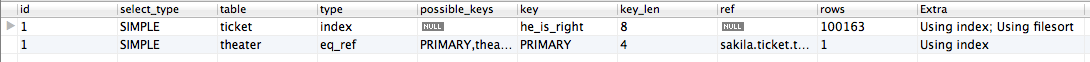
\includegraphics[width=1.0\columnwidth]{query_6} 
\end{figure}

This time MySQL optimizer used he\_is\_right index. It's because all data MySQL needs (theater\_id and price) to perform JOIN was stored in index structure.

\end{homeworkProblem}

\end{document}